\documentclass{article}
\usepackage[utf8]{inputenc}
\usepackage{listings}
\usepackage{graphicx}
\usepackage{float}
\usepackage{enumitem}

\setlength{\parindent}{0pt}
\lstset{
    basicstyle=\ttfamily\footnotesize,
    frame=single,
    xleftmargin=4pt,
    xrightmargin=4pt,
    breaklines=true
}

\title{Cloud Temperature \& Humidity Notification System}
\author{Lue Xiong}

\begin{document}

\maketitle
\newpage

\tableofcontents
\newpage

\obeylines

\section{Context}
The Cloud Temperature \& Humidity Notification System is about an IoT system that gives the ability to notify users of temperature and humidity fluctuations within their living environment through the usage of a Simple Message Service, which is also known as SMS. The system will also notify a user if the Particle Argon is offline by checking that data is being sent and stored in the database. Though this is the main concern of the system, it also allows users to visualize their daily climate averages in an interactive graph. The graph is automatically updated for the users to view whenever they want to on the web. Behind the scenes, most computation is abstracted away from the user by using Google Cloud Platform. The initiation of these functionalities start from the ambient temperature and relative humidity readings being published by the Particle Argon.\\

Working within the limitations of a small apartment and time allotted for the project, I cannot realize the full potential of the system. This project represents a single IoT device that enacts the above-mentioned functionalities. One can imagine, however, being able to send in-home area location data and climate readings with a multiple of these IoT devices scattered across a home with multiple rooms and stories. A user would be notified where in the house and when the climate has reached configured threshold levels for each device. They would then be able to see data points for each specified area of the home. Ideally, aspects of the system such as climate data publishing intervals, setting climate threshold and maximum notification intervals, and timezones should be configurable. With that said, the project seeks a minimum viable product. That is, the system will notify users of climate thresholds being met and device status through SMS notification as well as graphing average climate per day for viewing averages over days. User configuration will be beyond the minimum viable product as it would require additional development of a mobile or web application.\\

Though the system is targeted for the home living environment, it can be used for environments that require careful monitoring. Take a fermented product like kombucha for instance; it needs to be fermented in an environment where the ambient temperature hovers in the range of 65 to 85 degrees Fahrenheit over a week to multiple weeks. Low temperatures will either stop or dramatically slow down the fermentation process. High temperatures will quicken the fermentation process but also increases the risk of unwanted bacteria or mold growth that would ruin the product. Striking a balance with temperature for optimal conditions is difficult without information. The usage is only limited to the imagination.

\section{Problem}
The problem trying to be solved is giving the user climate data about their living environment. Certain ranges of temperature and humidity affect humans in ways that are detrimental to their health. For example, low humidity environments --characterized as 30\% relative humidity and below -- is a condition for being prone to respiratory infections, dry eyes, and itchy irritated skin. High humidity environments -- characterized as 60\% and above -- is a condition for bacterial and mold growth, a catalyst for the decomposition of organic materials, and the attraction of bugs and insects to the home. A way to solve that problem is to give a renter or homeowner actionable data to understand that their living environment needs change. That is where the Cloud Temperature \& Humidity Notification System comes in.

\section{Market Research}
From market researching, there are a couple of products that have similar functionalities:

\begin{itemize}
    \item AcuRite 01166M 3-Sensor Indoor Monitoring
    \item Govee Temperature Humidity Monitor
    \item Proteus AMBIO
\end{itemize}

All three of these products measure temperature and humidity and have their value propositions. We'll take a look at what they do and how they differ from this system.

\subsection{AcuRite 01166M 3-Sensor Indoor Monitoring}
AcuRite 1166M is packaged with 3 sensor units along with what they call a \textit{smartHUB}. The name is self-explanatory, it is the central communication piece for the 3 sensors. The max connection capacity for the smartHUB is 10 sensors. These sensors will read in the climate information of the environment and send it over to the smartHUB, which will then send information over the network to be processed and viewed online. There are some inherent flaws with this system as I will explain.\\

With the max capacity being 10 sensors connected to the smartHUB, it is only usable in a home environment and even then, a user may want more sensors if they have a larger home. The reason for the limitation is the design of having sensors centered around the smartHUB, and not standalone pieces that can interact with a network. The sensors are nothing without the smartHUB, therefore renders the system useless if it breaks. It also adds one more layer of complexity that is unnecessary for the user. Unnecessary because it is not doing anything complex enough to justify a central hub.

Another issue is reliability. The range at which these sensors can communicate with the smartHUB is limited and depending on the structure, materials, and size of the home can make it more difficult to reliably transfer information from sensor to hub. This issue of reliability is further enforced by users of the system.

\subsection{Govee Temperature Humidity Monitor}
\subsection{Proteus AMBIO}

\section{System Overview}
\label{section:overview}
This section will describe the minimum viable product requirements and the architectural decision made for achieving the desired results of the system.

\subsection{System Requirements}
To satisfy the need of giving a user useful information about temperature and humidity in their targeted environment, the following are the minimum viable product requirements:

\begin{itemize}
    \item All notifications sent to the user shall be an SMS message
    \item Notifications sent to the user shall be based on the following criteria
          \begin{itemize}
              \item Temperature upper threshold shall be set to lesser than or equal to 75 degrees Fahrenheit
              \item Temperature lower threshold shall be set to greater than or equal to 65 degrees Fahrenheit
              \item Humidity upper threshold shall be set to lesser than or equal to 60 percent relative humidity
              \item Humidity lower threshold shall be set to greater than or equal to 30 percent relative humidity
          \end{itemize}
    \item Minimum 1-hour gap in between each SMS message per climate type (AKA temperature and humidity) reaching above or below the threshold value
    \item Check device status every hour
    \item
\end{itemize}

\subsection{Event-Driven Architecture}
The approach taken for the system as mentioned before is heavy on the software side which manifests into an event-driven serverless architecture. An event-driven serverless architecture in the system context allows the climate data readings to be sent as events, processed based on its event type, and have actions performed without the need for standing up servers. The following are benefits of the said architecture:

\begin{itemize}
    \item Loose coupling between software components
    \item Automatically scale based on user demand
    \item All processing is driven by events
    \item No need for management of servers
    \item Inherent stateless nature
    \item Overall cost reduction versus managed servers
\end{itemize}

While these benefits are good to have, every architectural decision has its drawbacks. The following  are drawbacks of the said architecture:

\begin{itemize}
    \item Each serverless function must provide its own packaged dependencies
    \item Having a large number of serverless functions can become unwieldy
    \item Long-running processes are not fit for serverless functions
    \item Handling system state amongst stateless functions can be tricky
\end{itemize}

Using an event-driven serverless architecture made sense for this system, as the needs of the system are fulfilled automatically on publishing data without any manual intervention.

\section{Process and Implementation}
I will preface that the Cloud Temperature \& Humidity Notification System is heavily software-based. The hardware components are nothing special and ultimately serve as a vessel for sending climate information to be processed in the cloud to create the closed-feedback loop. The Particle Argon referenced in Section~\ref{section:hardware} will contain firmware that is fundamental to the system requirements and architectural decision in Section~\ref{section:overview}. This particular section will describe the thought process behind the implementation, considerations taken during development, and how the system performs user notification and automatic graph updates.

\subsection{Hardware Components}
\label{section:hardware}
\begin{figure}[H]
    \center
    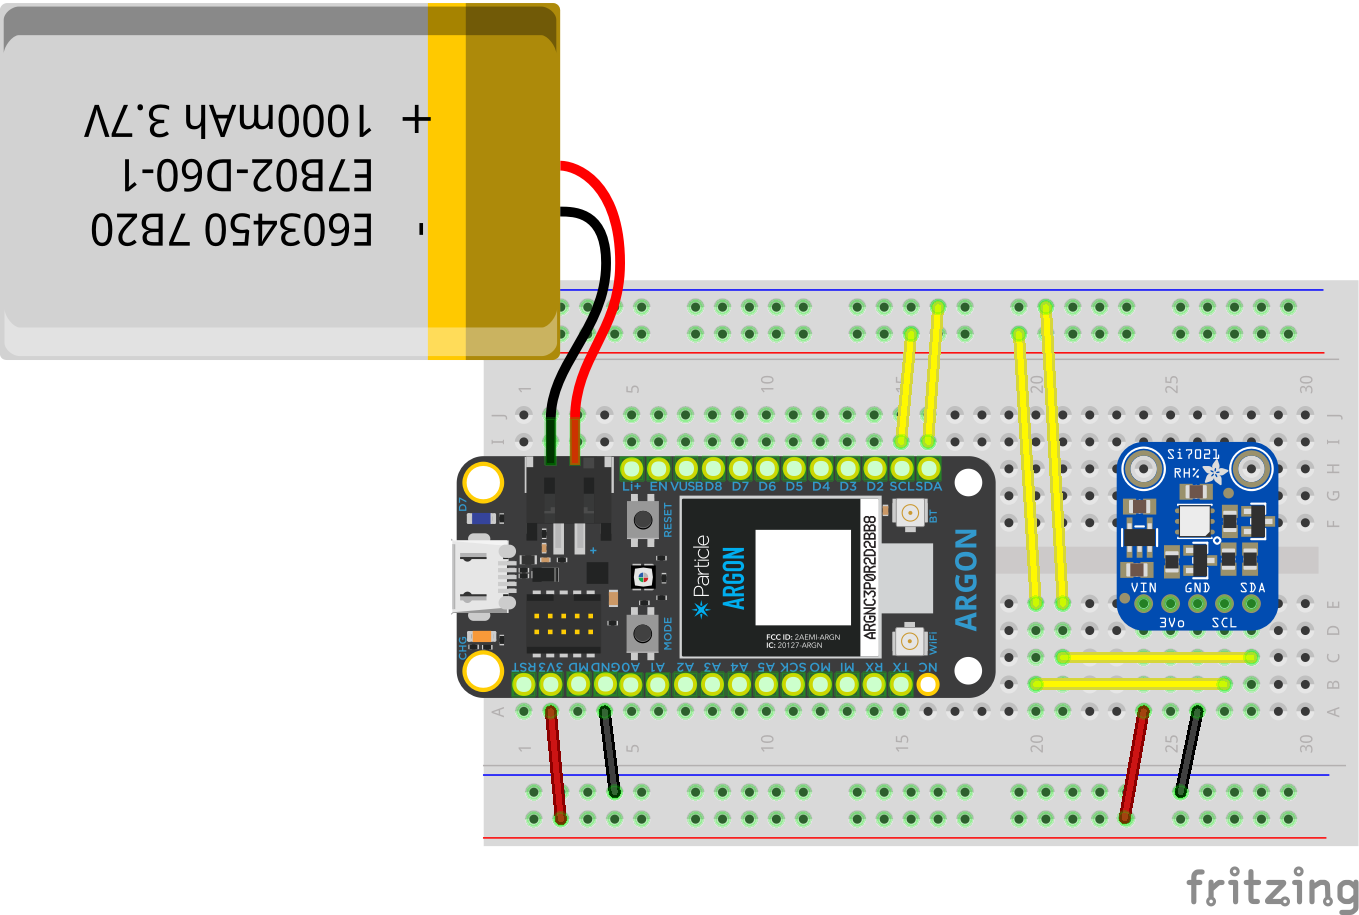
\includegraphics[width=\textwidth]{images/breadboard-schematic.png}
    \caption{Breadboard Schematic}
    \label{fig:breadboard_schematic}
\end{figure}

Figure~\ref{fig:breadboard_schematic} comprises the following hardware components:

\begin{itemize}
    \item Particle Argon — IoT development kit for connecting and sending information over the network
    \item Adafruit Si7021 — Temperature and humidity sensor breakout board
    \item Breadboard — Base to create circuits and prototype electronics
    \item Jumper Wires — Cables able to connect components
    \item Lithium Ion Polymer Battery 1000 mAh — A power source for the connected components
\end{itemize}

\newpage

\subsection{Particle Argon and Particle Cloud}
Particle Argon is flashed with firmware written with C code. It is used with Particle's API and the Adafruit Si7021 helper library. Understanding the Particle ecosystem's role in the system will reveal the scope of its interactions in the event-driven serverless architectural decision.

\begin{minipage}[c]{\textwidth}
    \begin{figure}[H]
        \lstinputlisting[language=C,firstline=9,lastline=12]{../src/particle-argon-temperature-humidity.ino}
        \caption{setup() function}
        \label{fig:setup}
    \end{figure}
\end{minipage}\ \\\\

The \textbf{setup()} as shown in Figure~\ref{fig:setup} is important here for two reasons. The first part is that the Particle Argon is in default timezone of Universal Time Coordinated (UTC) which differs from the timezone I live in is Central Daylight Time (CDT). To be able to represent the timezone difference, setting the default timezone with an offset of minus 5 hours is required. The second part is making sure that the Adafruit Si7021 is enabled after being initialized because it is the central piece for reading ambient temperature and relative humidity from a given environment.

\begin{minipage}[c]{\textwidth}
    \begin{figure}[H]
        \lstinputlisting[language=C,firstline=14,lastline=37]{../src/particle-argon-temperature-humidity.ino}
        \caption{loop() function}
        \label{fig:loop}
    \end{figure}
\end{minipage}\ \\\\

In Figure~\ref{fig:loop}, the \textbf{loop()} function shows that temperature and humidity are being read with the sensor object. They are then used as values to publish to the Particle Cloud. From that point on they are passed to Google Cloud Platform. However, there will be a further explanation of how this integration works and what processes happen on the Google Cloud Platform in Section~\ref{section:gcp}.

\begin{minipage}[c]{\textwidth}
    \begin{figure}[H]
        \lstinputlisting[language=C,firstline=39,lastline=55]{../src/particle-argon-temperature-humidity.ino}
        \caption{isEndOfDay() function}
        \label{fig:endofday}
    \end{figure}
\end{minipage}\ \\\\

Beyond publishing the climate values, the \textbf{loop()} function checks whether the day has ended from the perspective of the system. The end of the day is defined as code in Figure~\ref{fig:endofday}. Before it was mentioned that a UTC offset of minus 5 hours was applied in the \textbf{setup()} function, and this is where it comes into context. The end of the day is 9 PM CDT, which is equivalent to 21 in a 24-hour format. Once the system understands that it is the end of the day, an event is published to update a file containing daily climate average aggregates for the day. To understand the update itself will require digging into the Google Cloud Platform integration. As written before, this will be further explained in Section~\ref{section:gcp}.\\

Concerning the end of the day as well as a variable called \textbf{publishIntervalMilliseconds} will be set to 1800000, in other words, 30 minutes. This publishing interval will last for 9 hours starting from 9 PM CDT to 6 AM CDT. During the working day, the \textbf{publishIntervalMilliseconds} is set to 900000, or 15 minutes. This plays a role in conserving battery because, during the night, it is only publishing climate data two per hour as opposed to four. However, the bigger battery-saving impact comes from placing the Particle Argon in a sleeping state.\\

A sleeping state means that the Particle Argon turns off all unnecessary internal processes that consume energy and maintains a low-power state for a duration of a configured time. There are two main modes of sleep state that Particle Argon can go into: \textbf{STOP} and \textbf{HIBERNATE}. The decision was to use the \textbf{STOP} sleeping mode because it provides the opportunity to keep the network connection alive while it is in a low-power state. \textbf{HIBERNATE} does not allow this, and if it was used, it would require the Particle Argon to completely establish a new connection every time it wakes up from the specified duration of \textbf{publishIntervalMilliseconds}; defeating the point of using it.

\subsection{Google Cloud Platform and Peripherals}
\label{section:gcp}
Google Cloud Platform is the most important part of the whole system. That being said, it is also important to outline the purpose of each tool used within the platform.\\

\textbf{Compute Engine}
\textbf{Firestore}
\textbf{Functions}
\textbf{IAM}
\textbf{PubSub}
\textbf{Scheduler}
\textbf{Secret Manager}
\textbf{Storage}

\subsubsection{SMS Notification}

\subsubsection{Climate Data Graph}

\section{Discussion}
It was quite a difficult experience integrating all the hardware and technology stack used in the Cloud Temperature \& Humidity Notification System. This was especially true of Google Cloud Platform because while there was extensive documentation on their tools, Google is a company known for renaming, rebranding, and deploying new tools often. As one can imagine, that makes it difficult to discern what was changed, what to look for, and what to use. Their documentation is not very well organized as concepts and subconcepts of a particular tool are scattered throughout the website. Ironically enough, it was more efficient -- though not exactly pleasant -- to Google search for what I needed than navigating through the Google Cloud Platform documentation.\\

Aside from the obvious pitfall of the documentation, Google Cloud Platform is powerful in what it can do for software. 

\section{Conclusion}

\end{document}
